%% 
%% Copyright 2019-2020 Elsevier Ltd
%% 
%% This file is part of the 'CAS Bundle'.
%% --------------------------------------
%% 
%% It may be distributed under the conditions of the LaTeX Project Public
%% License, either version 1.2 of this license or (at your option) any
%% later version.  The latest version of this license is in
%%    http://www.latex-project.org/lppl.txt
%% and version 1.2 or later is part of all distributions of LaTeX
%% version 1999/12/01 or later.
%% 
%% The list of all files belonging to the 'CAS Bundle' is
%% given in the file `manifest.txt'.
%% 
%% Template article for cas-dc documentclass for 
%% double column output.

\documentclass[a4paper,fleqn]{cas-dc}
\usepackage[authoryear,longnamesfirst]{natbib}


\begin{document}
\let\WriteBookmarks\relax
\def\floatpagepagefraction{1}
\def\textpagefraction{.001}

\shorttitle{Analiza zbioru pacjętów z SM chorych na COVID-19 modelem One-CLass SVM}

\shortauthors{}

\title [mode = title]{Analiza zbioru danych "Patient-level dataset to study the effect of COVID-19 in people with Multiple Sclerosis" z wykorzystaniem nadzorowanego algorytmu uczenia maszynowego One-Class SVM(Support Vector Machines)}                      

\author{Anna Mrozek, Bartosz Panek \,i\, Przemysław Jura  }

\renewcommand{\abstractname}{STRESZCZENIE}
\begin{abstract}
Artykuł analizuje zbiór danych pacjentów ze stwardnieniem rozsianym (SM), którzy przeszli COVID-19, przy użyciu nadzorowanego algorytmu One-Class SVM. Celem jest identyfikacja przypadków o zwiększonym ryzyku ciężkiego przebiegu infekcji. Umożliwi to zidentyfikowanie charakterystycznych cech pacjentów bardziej narażonych na powikłania.
\end{abstract}

\renewcommand{\abstractname}{STRESZCZENIE}
\begin{keywords}
One-Class SVM \sep COVID-19 
\end{keywords}

\maketitle

\section{Wprowadzenie}
Pandemia COVID-19 miała znaczący wpływ na osoby z chorobami przewlekłymi, w tym na pacjentów ze stwardnieniem rozsianym (SM). SM jest przewlekłą chorobą autoimmunologiczną, która wpływa na układ nerwowy i może prowadzić do trwałego uszkodzenia neuronów oraz ograniczenia funkcji motorycznych oraz poznawczych przez uszkodzenia mieliny oraz włókien nerwowych [1][2][3] Osoby z MS są bardziej podatne na infekcje z powodu złożonego działania samej choroby, jej leczenia i naturalnego przebiegu [4].  Ze względu na charakter choroby i stosowane terapie immunosupresyjne, pacjenci z SM mogą być bardziej narażeni na cięższy przebieg infekcji wirusowych, w tym COVID-19.[5][6] 

Analiza danych od pacjentów z SM, którzy przeszli COVID-19, może dostarczyć ważnych informacji na temat ryzyka powikłań i zidentyfikować czynniki przyczyniające się do poważniejszych objawów, co ostatecznie może pomóc w lepszym monitorowaniu i opiece nad tą grupą pacjentów.

\section{Cel}
Celem badania jest wykorzystanie nadzorowanego algorytmu One-Class SVM do analizy zbioru danych pacjentów ze stwardnieniem rozsianym, którzy przeszli COVID-19, w celu zidentyfikowania cech pacjentów o zwiększonym ryzyku ciężkiej infekcji. Oczekuje się, że wyniki analizy dostarczą wskazówek do opracowania bardziej ukierunkowanych strategii opieki i środków zapobiegawczych dla pacjentów ze stwardnieniem rozsianym w kontekście potencjalnych przyszłych pandemii lub innych zagrożeń wirusowych.

\section{Przegląd literatry}
W literaturze medycznej i naukowej, od początku pandemii COVID-19, wiele badań skupiało się na analizie wpływu wirusa SARS-CoV-2 na osoby cierpiące na choroby przewlekłe i autoimmunologiczne, takie jak stwardnienie rozsiane (SM). Wyniki tych badań sugerują, że pacjenci z SM, zwłaszcza ci stosujący terapie immunosupresyjne, mogą być bardziej narażeni na cięższy przebieg COVID-19 oraz związane z nim powikłania[7][8]. U pacjentów z SM często obserwuje się obniżoną odporność oraz większą podatność na infekcje, co wynika zarówno z samej choroby, jak i z efektów leków tłumiących układ odpornościowy[9]. Dodatkowo w badaniach zwraca się uwagę na takie czynniki ryzyka jak wiek, płeć, rodzaj stosowanego leczenia oraz inne choroby towarzyszące, które mogą zwiększać ryzyko ciężkiego przebiegu infekcji u tej grupy pacjentów.

W ostatnich latach coraz większą popularność zyskuje zastosowanie algorytmów uczenia maszynowego, takich jak Support Vector Machines (SVM), do analizy danych medycznych. Algorytmy te pozwalają na wykrywanie wzorców i anomalii w dużych, zróżnicowanych zbiorach danych[10]. W szczególności algorytm One-Class SVM, używany do wykrywania anomalii, jest przydatny do identyfikacji przypadków wysokiego ryzyka w danych medycznych, gdzie przypadki nietypowe (np. pacjenci bardziej narażeni na ciężki przebieg COVID-19) występują rzadko. Badania pokazują, że One-Class SVM dobrze sprawdza się w analizie populacji pacjentów, gdy dostęp do dużych zbiorów danych o przypadkach zdrowych jest ograniczony, co często stanowi wyzwanie w analizie medycznej[11].

W kontekście badań nad COVID-19 i SM, algorytmy nadzorowanego uczenia maszynowego, takie jak SVM, umożliwiają dokładniejszą analizę czynników ryzyka oraz lepsze prognozowanie ciężkiego przebiegu choroby. Wyniki takich analiz mogą być przydatne nie tylko dla lekarzy, ale także dla decydentów zajmujących się zdrowiem publicznym, ponieważ pozwalają na opracowanie bardziej ukie-runkowanych strategii opieki dla osób z SM, które są bardziej narażone na zagrożenia związane z wirusami, takimi jak COVID-19.

\section{Metodologia}
W badaniu zastosowano algorytm nadzorowanego ucze-nia maszynowego One-Class SVM w celu identyfikacji pacjentów z podwyższonym ryzykiem ciężkiego przebiegu COVID-19 w grupie osób ze stwardnieniem rozsianym. Analiza obejmowała cechy kliniczne pacjentów, takie jak wiek, płeć, typ leczenia oraz choroby współistniejące, aby zidentyfikować wzorce związane z większą podatnością na powikłania.

\subsection{Dataset}
Z inicjatywy MS Global Data Sharing Initiative (GDSI) zbadano, jak leki immunosupresyjne lub immunomodulujące wpływają na COVID-19 i jego przebieg u osób z MS. GDSI miała na celu zwiększenie skali zbierania danych dotyczących COVID-19 i dostarczenie społeczności związanej z MS informacji opartych na danych podczas pandemii [12]. W ramach GDSI wybrano kluczowe zmienne obejmujące informacje o COVID-19, stopniu jego ciężkości, leczeniu, dane demograficzne, historię i nasilenie MS, stosowanie leków modyfikujących przebieg choroby (DMT), choroby współistniejące i wybrane zachowania związane ze stylem życia, takie jak palenie tytoniu. Globalna społeczność MS współpracowała, przekazując dokumentację statusu COVID-19 u osób z MS za pośrednictwem centralnej platformy udostępnionej przez QMENTA [13].

Ten zbiór danych został zebrany za pomocą narzędzia do szybkiego wprowadzania danych, które umożliwiało klinicystom, osobom ze stwardnieniem rozsianym (PwMS) lub ich przedstawicielom bezpośrednie wprowadzanie informacji do centralnej platformy GDSI. Narzędzie to zawierało kwestionariusz oparty na wcześniej ustalonych zmiennych i nie gromadziło bezpośrednich danych osobowych, aby chronić prywatność użytkowników. Narzędzie zostało wyłączone 3 lutego 2022 roku.

Zbiór danych obejmuje informacje o 1141 osobach ze stwardnieniem rozsianym (PwMS). Aby zapewnić zgodność danych z wytycznymi HIPAA, przeprowadzono proces deidentyfikacji. 

Ponieważ w danych nie zbierano imion pacjentów, deidentyfikacja skupiła się na datach i wieku pacjentów. Daty w kolumnie „stop-or-end-date-combined” zostały przesunięte o losową liczbę dni (między -15 a 15), aby uniemożliwić identyfikację na podstawie dat. Wiek pacjentów sklasyfikowano w cztery grupy: 0 dla osób w wieku 0–17 lat, 1 dla osób między 18 a 50 lat, 2 dla osób między 51 a 70 lat, oraz 3 dla osób powyżej 71 lat. Dzięki temu żadne dokładne wartości wieku powyżej 90 lat nie zostały ujawnione. Po klasyfikacji zmiennych i wdrożeniu odpowiednich środków ostrożności dane zostały zdeidentyfikowane i spełniają standardy HIPAA, zachowując jednocześnie wartość badawczą. Ponadto, aby zapewnić ochronę prywatności, zastosowano techniki takie jak Kanonimizacja oraz różnorodność.

Zbiór danych obejmuje zestaw z góry określonych zmiennych, takich jak płeć, kategoria wiekowa, typ MS, wynik EDSS, status palenia oraz kategoria BMI. Te zmienne dostarczają informacji o demografii pacjentów, ich stanie klinicznym oraz symptomach związanych z COVID-19. 

\subsection{Opis metody}
Jednoklasowy SVM (One-Class Support Vector Machine, OCSVM) to algorytm przeznaczony do wykrywania anomalii w zbiorze danych. Zamiast klasyfikować dane do dwóch lub więcej klas, jak w klasycznym SVM, OCSVM koncentruje się wyłącznie na danych normalnych.[14][15] Jego celem jest zbudowanie granicy wokół większości przypadków normalnych, tworząc "strefę normalności", która odróżnia standardowe przypadki od anomalii.

Główna zasada działania OCSVM opiera się na maksymalizacji marginesu między przypadkami normalnymi a granicą, która oddziela normę od anomalii. Dzięki temu model lepiej rozpoznaje dane odstające, które znajdują się poza wyznaczoną strefą.[16][17]

Kluczowym elementem działania OCSVM jest funkcja decyzyjna oparta na hiperpłaszczyźnie, która oddziela dane od początku układu współrzędnych. Wzór na hiperpłaszczy-znę wyrażany jest jako:
\begin{equation}
    f(x) = \mathbf{w} \cdot x - \rho
\end{equation}
gdzie:
\begin{itemize}
\setlength\itemsep{0px}
    \item w – wektor normalny do hiperpłaszczyzny, wyznaczony podczas procesu uczenia,
    \item  x – próbka danych,
    \item  $\rho$ – jest wartością progową (bias), która definiuje margines.
\end{itemize}


\par OCSVM posiada szereg parametrów, dzięki którym możliwe jest dostosowywanie modelu do specyficznych potrzeb:

\begin{itemize}
    \item \textbf{Parametr $\nu$}: Kontroluje liczbę obserwacji uznawa-nych za anomalie. Parametr ten przyjmuje wartości w przedziale od 0 do 1 i determinuje udział anomalii, jakie model może tolerować w zbiorze treningowym (np. jeśli $\nu$ = 0.05, oznacza to, że około 5\% próbek zostanie sklasyfikowanych jako anomalie).
    \item \textbf{Parametr $\gamma$}: Wpływa na kształt granicy decyzyjnej poprzez dopasowywanie modelu do danych. Mniejsza wartość $\gamma$ oznacza „szerszą” granicę, obejmującą więcej punktów, natomiast większa wartość $\gamma$ powo-duje, że granica jest bardziej dopasowana do danych, co może zwiększać ryzyko nadmiernego dopasowania (overfitting).
    \item \textbf{Jądro (\textit{ang. kernel})}: One-Class SVM często wykorzystuje funkcje jądrowe, aby modelować nieliniowe granice decyzyjne i lepiej dopasować się do danych, które nie są liniowo rozdzielne w przestrzeni cech. Wybór jądra, zwany również „sztuczką jądra”, \break wpływa na charakter dopasowania modelu i jego wydajność.
\end{itemize}

Podczas treningu OCSVM analizuje wyłącznie dane normalne, co sprawia, że jest szczególnie użyteczny w sytuacjach, gdy anomalie są rzadkie lub trudne do zidentyfikowania. Model staje się wtedy bardziej niezawodny w rzeczywistych zastosowaniach, takich jak wykrywanie oszustw, monitorowanie awarii czy zabezpieczanie sieci komputerowych. OCSVM może wykorzystać różne funkcje jądra, co umożliwia mu wykrywanie zarówno prostych, jak i bardziej złożonych odchyleń.[18]

\subsection{Opis przeprowadzonych obliczeń}

1. Przygotowanie i czyszczenie danych - rozpoczęliśmy od wczytania danych oraz wybrania interesujących nas cech, które następnie zostały przekształcone w sposób umożliwiający przeprowadzenie obliczeń:
\begin{itemize} 
\item Dla kolumn binarnych (yes/no) wartości zostały zamienione na liczby 0 i 1.
\item  Dla kolumn kategorycznych i ordinalnych (np. age-in-cat, covid19-outcome-levels-2, report-source) zostały przypisane wartości liczbowe, zgodnie z przyjętym mapowaniem.
 \item Brakujące wartości w danych zostały wypełnione zerami, co pozwoliło na uniknięcie problemów podczas analizy i treningu modelu.
\end{itemize}

2. Tworzenie nowych zmiennych: symptom-score oraz comorbidity-score, aby skonsolidować informacje o objawach i chorobach współistniejących.
\begin{itemize} 
\item Stworzyliśmy dwie kolumny symptom-score oraz comorbidity-score, które zliczają ilość objawów wirusa COVID-19 oraz liczby chorób współistniejących dla każdego pacjenta.
\item  Kolumny te były następnie skalowane przy użyciu StandardScaler, co pozwala na lepszą interpretację wyników oraz standaryzację w zakresie modelowania.
\end{itemize}
Efektem było, uzyskanie wartości numerycznych, które reprezentują intensywność symptomów oraz liczbę chorób współistniejących dla każdego pacjenta.


3. Dane zostały podzielone na zbiór treningowy (X\_train) i testowy (X\_test) za pomocą funkcji train\_test\_split z biblioteki sklearn, przy czym 70\% danych przydzielono do zbioru treningowego. Zbiór treningowy służy do uczenia modelu, natomiast testowy został rozszerzony do wszystkich danych, więc zawierał w sobie nowe nieznane dane dla modelu, jak i poprzednie dane. Wynikało to z łatwiejszego testowania danych, a wyniki i wnioski pozostawły podobne, a nawet lepsze po obserwacji, wynikało to miętzy innymi z większej próby. Ustawienie argumentu random\_state=42 zapewnia reprodukowalność wyników, dzięki czemu podział danych jest zawsze taki sam przy kolejnych uruchomieniach. Warto zaznaczyć, iż na potrzeby dalszej oceny modelu pacjęci hospitalizowani zostali uznani za anomalie ponieważ najciężej przeszli chorobę (ok. 2\%). Dlatego do nauki modelu zostali wykorzystani jedynie pacjęci nie hospitalizowani, w celu nauczeniu danych na danych normalnych. 

4. Trening modelu One-Class SVM - zastosowaliśmy algorytm One-Class Support Vector Machine (SVM) z jądrem rbf, który dobrze radzi sobie z modelowaniem nieliniowych granic decyzyjnych. Model trenowano, aby rozpoznawał typowe cechy pacjentów COVID-19 i SM, a następnie by przewidywał, które próbki są podobne do tego wzorca, a które mogą być anomaliami. Po treningu model przypisywał każdej próbce etykietę 1 (normalna) lub -1 (anomalia). Próbki oznaczone jako anomalia zawarto w nowej ramce anomalies w celu dalszej analizy. Model trenowano na różnych parametrach, czy to wielkości przyjętych anomali, kształtu granicy decyzyjnej czy współczynnika jądra. Najlepsze wyniki osiągał dla przyjętych 2\% anomali i współ-czynnika jądra 'scale'.

5. Analiza wyników - na podstawie wykrytych anomalii przeprowadziliśmy szereg analiz, tworząc wizualizacje, które pomagają zrozumieć charakterystykę anomalii[19]

\subsection{Wykorzystane metryki oceny}


\textbf{Raport klasyfikacji (ang. classification report)} to podsumowanie wyników modelu klasyfikacyjnego, które przedstawia kluczowe metryki takie jak precyzja (precision), czułość (recall), i F1-score dla każdej klasy. Precyzja wskazuje, jak wiele z klasyfikacji pozytywnych jest poprawnych, podczas gdy czułość pokazuje, ile przykładów rzeczywiście pozytywnych zostało poprawnie sklasyfikowa-nych. F1-score jest średnią harmoniczną precyzji i czułości, co sprawia, że dobrze nadaje się do oceny modeli na danych niezbalansowanych. Raport zawiera również wskaźnik wsparcia (support), który pokazuje liczbę przykładów w każdej klasie.

\textbf{Dokładność}, inaczej zwana accuracy, to stosunek liczby poprawnych predykcji (zarówno pozytywnych, jak i negatywnych) do całkowitej liczby przykładów w danych testowych. Jest to ogólny wskaźnik skuteczności modelu. Jednak w przypadku danych niezbalansowanych, dokładność może być myląca, ponieważ wysoka wartość może wynikać z dominacji jednej klasy. Dlatego warto uzupełniać analizę dokładności bardziej szczegółowymi metrykami, jak np. F1-score czy False Positive Rate.

\textbf{Funkcja decyzyjna (ang. decision\_function)} w modelach takich jak One-Class SVM określa odległość przy-kładów od granicy decyzyjnej modelu. Wyniki funkcji decyzyjnej wskazują, na ile pewnie model klasyfikuje przykład jako normalny lub anomalię. Wartości dodatnie sugerują, że przykład jest wewnątrz granicy klasy normalnej, a wartości ujemne sugerują, że przykład jest anomalią. Wartości bliżej zera oznaczają, że przykład znajduje się blisko granicy decyzyjnej.

\textbf{Odsetek anomalii} określa, jaka część danych została sklasyfikowana jako anomalie przez model. W modelach takich jak One-Class SVM parametr nu kontroluje, jaki procent danych jest uważany za anomalie podczas trenowania modelu. Jeśli odsetek anomalii w wynikach jest znacznie wyższy niż zakładany, może to oznaczać nadmierną surowość modelu. Z kolei zbyt niski odsetek może sugerować, że model nie wykrywa rzeczywistych anomalii.

\textbf{False Positive Rate (FPR)} to wskaźnik fałszywych alarmów, obliczany jako stosunek liczby fałszywie pozytywnych klasyfikacji (FP) do liczby wszystkich rzeczywistych przykładów negatywnych (FP + TN). Wysoki FPR oznacza, że model często błędnie klasyfikuje normalne przypadki jako anomalie, co może być problematyczne w zastosowaniach wymagających dużej precyzji (np. w diagnostyce medycznej). Zmniejszenie FPR można osiągnąć przez odpowiednie dostrojenie parametrów modelu lub zmianę progu decyzyjnego.

\section{Wyniki}

\subsection{Ocena modelu One-Class SVM}

\begin{figure}[h]
	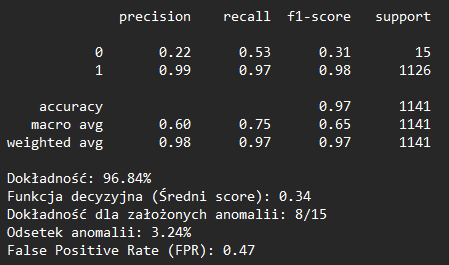
\includegraphics[scale=.70]{wykresy/ocena1.png}
	\caption{Ocena modelu One-class SVM}
	\label{FIG:1}
\end{figure}

\begin{figure}[h]
	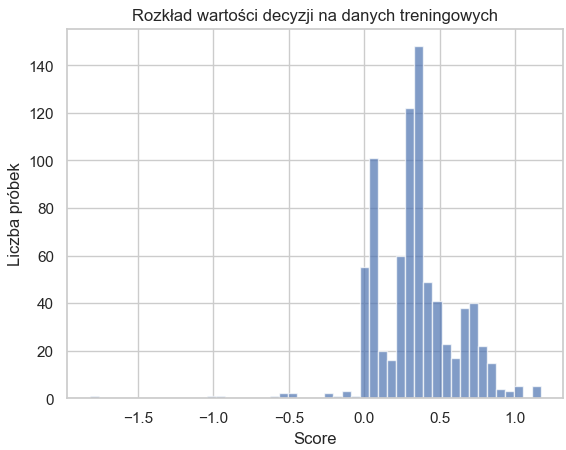
\includegraphics[scale=.66]{wykresy/ocena2.png}
	\caption{Rozkład wartości decyzji dla danych modelu One-class SVM}
	\label{FIG:1}
\end{figure}


\textbf{Na potrzeby ocenienia modelu, zostały wyodrębnione potencjalne dane które prawdopodobnie były anomaliami to znaczy przypadkami, które wymagały hospitalizacji i poważniejszego leczenia. To właśnie ta grupa osób została uznana za tą która najcieżej przeszła chorobę. Za potencjalne anomalie zostaly uznane przypadki, które w danych w kolumnie covid19\_admission\_hospital zawierały informacjie o  hospitalizacji. Dodatkowo fakt, iż jedynie ok 2\% osób badanych trafiło do szpitala potwier-dzało założenie, że to właśnie tam należy doszukiwać się potencjanych anomali.}  

Model klasyfikacyjny został oceniony na podstawie kilku metryk, takich jak precyzja (precision), czułość (recall), F1-score, oraz wsparcie (support). Dla klasy 0 (anomalia) precyzja wyniosła 0.22, co oznacza, że jedynie 22\% przypadków sklasyfikowanych jako anomalie było popraw-nych. Czułość wyniosła 0.53, co wskazuje, że model wykrył 53\% rzeczywistych anomalii. Niski F1-score (0.31) podkreśla trudności modelu w skutecznym identyfikowaniu anomalii, co jest szczególnie problematyczne przy tylko 15 przykładach rzeczywistych anomalii (support). Dla klasy 1 (normalny przypadek), wyniki są bardzo wysokie – precyzja 0.99 i czułość 0.97 świadczą o dużej skuteczności modelu w identyfikacji normalnych przypadków, co znajduje odzwierciedlenie w wysokim F1-score równym 0.98. Średnia dokładność modelu (accuracy) wyniosła 96.84\%, co sugeruje ogólną skuteczność klasyfikacji, ale maskuje problem niskiej wydajności w detekcji anomalii.

Odsetek anomalii w zbiorze danych wynosi 3.24\%, co wskazuje na dużą nierównowagę klas. False Positive Rate (FPR) na poziomie 0.47 oznacza, że model często błędnie klasyfikuje normalne przypadki jako anomalie. Dodatkowo, średni wynik na danych testowych z funkcji decyzyjnej wyniósł 0.34, co wskazuje, że większość przy-kładów testowych znajduje się blisko granicy decyzyjnej modelu. To może sugerować, że model ma trudności z wyraźnym rozdzieleniem klas, szczególnie w przypadku anomalii.


\subsection{Wynik analizy}

 Wykresy znajdują się na końcu opracowania.


\section{Opis wyników}

Opis wynkresów znajdujących się na końcu opracowania:

Figure 3: Na wykresie widzimy histogram z liczbą próbek oznaczonych jako normalne i anomalia przez model One-Class SVM.
Z wykresu wynika, że większość próbek została sklasyfikowana jako normalne (oznaczone jako 1), podczas gdy mniejsza liczba próbek została uznana za anomalie.
Wysoka liczba normalnych próbek w stosunku do anomalii wskazuje, że model wykrywa anomalia rzadziej, co jest zgodne z celem detekcji anomalii, ponieważ anomalie rzadziej występują.


Figure 4: Histogram pokazuje, że większość przypadków anomalii ma niski symptom\_score, głównie na poziomie 0, z kilkoma przypadkami rozproszonymi na wyższych wartościach aż do 10. Niskie wartości mogą sugerować, że większość anomalii wykazuje niewiele lub żadnych symptomów, choć istnieją wyjątki, gdzie symptom score jest wyższy.


Figure 5: Histogram przedstawia, że większość anomalii ma comorbidity\_score równy zero, co oznacza brak chorób współistniejących, chociaż kilka przypadków posiada wyższe wartości aż do 4. To sugeruje, że choć wiele przypadków anomalii nie ma dodatkowych schorzeń, niektóre z nich charakteryzują się złożonymi chorobami współistniejącymi.


Figure 6: Histogram pokazuje rozkład Symptom\_score dla normalnych przypadków. Najwięcej przypadków ma symptom\_score wynoszący 0, ale przypadki są bardziej równomiernie rozproszone w przedziale od 1 do 7. Sugeruje to, że normalne przypadki mogą mieć różny poziom symptomów, ale głównie wyróżniają się skrajnie niskimi wartościami.


Figure 7: Tutaj widzimy, że większość przypadków normalnych ma comorbidity\_score bliski zero, choć niektóre przypadki osiągają wartość 1. Wskazuje to, że większość przypadków normalnych nie ma chorób współistniejących, ale mogą występować łagodne współistniejące schorzenia.

Figure 8: Na wykresie przedstawiono średnie wartości cech binarnych dla przypadków zaklasyfikowanych jako anomalie. Są to cechy, które wskazują obecność lub brak pewnych objawów lub stanów zdrowotnych. Wysokie średnie wartości wskazują na częstsze występowanie danej cechy wśród anomalii:
Najwyższe średnie wartości dotyczą cech takich jak current\_dmt (obecnie przyjmowana terapia modyfikująca chorobę), covid19\_self\_isolation (izolacja w związku z COVID-19), oraz covid19\_has\_symptoms (obecność symptomów COVID-19). Oznacza to, że osoby klasyfikowane jako anomalie często są poddane leczeniu, mają objawy lub były w izolacji.
Kolejne wysokie cechy to np. has\_comorbidities (choroby współistniejące) oraz różne objawy związane z COVID-19, takie jak dry\_cough (suchy kaszel) i fatigue (zmęczenie), co sugeruje, że anomalie mogą być powiązane z przypadkami COVID-19 lub innymi poważnymi objawami chorobowymi.

Figure 9: Na tym wykresie poziomym przedstawiono średnie wartości dla różnych cech binarnych w normalnych przypadkach (bez anomalii). Cecha o najwyższej średniej wartości to current\_dmt, co wskazuje, że pacjenci normalni często używają terapii modyfikujących chorobę (DMT). Inne często występujące cechy to current\_or\_former\_smoker oraz covid19\_self\_isolation, oraz covid19\_has\_symptoms, co sugeruje, że objawy COVID-19 i byli bądź obecni palacze t znaczna grupa osób w normalnej grupie.

Figure 10: Większość anomalii dotyczy osób młodszych (kategoria 1), co może sugerować, że młodsze osoby mają większe ryzyko występowania anomalii w danych.

Figure 11: Zdecydowana większość przypadków anomalii dotyczy osób z niższym BMI (kategoria 0), co może wskazywać na związek między BMI a nietypowymi przypadkami.

Figure 12: Wśród anomalii przeważają kobiety (kategoria 1), co sugeruje, że w danych kobiet częściej występują anomalie.

Figure 13: Większość anomalii dotyczy osób bez przypisania do ms\_type2 (kategoria 0), ale niektóre przypadki należą do kategorii 1 lub 2.

Figure 14: Rozkład wskazuje, że wśród anomalii dominują łagodniejsze wyniki COVID-19 (kategoria 0), choć są też przypadki umiarkowane (kategoria 1) i ciężkie (kategoria 2).

\section{Podsumowanie}
Zgromadzony zbiór danych liczył jedynie ponad 1100 przypadków, co w kontekście analiz statystycznych i uczenia maszynowego jest liczbą stosunkowo niewielką, szczególnie przy analizie złożonych zjawisk, takich jak przebieg COVID-19 w określonych populacjach. Dodatkowo dane te charakteryzowały się dużą ilością brakujących wartości – aż około 70\% przypadków zawierało znaczne luki w informacjach, co ograniczało ich użyteczność. Tylko 2\% przypadków dotyczyło osób hospitalizowanych, co dodatkowo zmniejszało wartość predykcyjną modelu, ponieważ ciężkie przypadki stanowiły bardzo niewielką część danych i były słabo reprezentowane.

Problemem była również nierównomierność rozkładu danych w kluczowych grupach, takich jak płeć i wiek, co prowadziło do stronniczości wyników. Na przykład, nierównomierna liczba kobiet i mężczyzn w próbie lub różnice w liczbie obserwacji pomiędzy grupami wiekowymi powodowały, że model mógł błędnie wyciągać wnioski na podstawie nadreprezentowanych cech. Brak równowagi w danych utrudniał także identyfikację rzeczywistych wzorców w populacji i prowadził do fałszywego postrzegania wiarygodności wyników.

Dodatkowym wyzwaniem w analizie takich danych jest specyfika COVID-19 jako choroby o niejasnych i zróżnicowanych objawach klinicznych. COVID-19 może manifestować się w bardzo szerokim spektrum od całkowicie bezobjawowego przebiegu, poprzez łagodne symptomy, aż po ciężkie przypadki wymagające hospitalizacji i intensywnej terapii. Ta zmienność znacząco utrudnia stworzenie jednorodnych wzorców klasyfikacyjnych, szczególnie gdy dane są ograniczone i niekompletne. W przypadku omawianego zbioru brak dostatecznej reprezentacji ciężkich przypadków oraz brak dokładnych informacji o objawach dodatkowo ograniczał możliwość identyfikacji kluczowych cech różnicujących normalne przypadki od anomalii.

W tych okolicznościach zastosowanie modelu one-class SVM nie było właściwym podejściem. Model ten zakłada, że dostępne dane normalne są wystarczająco reprezentatywne, by umożliwić wykrycie anomalii. Jednakże w tym przypadku, z powodu małej liczby przypadków, braku wystarczających przykładów rzeczywistych anomalii (np. ciężkich przypadków COVID-19), a także braków danych i ich nierównomiernego rozkładu, model nie był w stanie skutecznie odróżnić anomalii od danych normalnych. W konsekwencji one-class SVM wykazał fałszywie wyniki.

\textbf{Podsumowując, niedostateczna liczba przypadków, liczne braki danych, nierównomierność ich rozkładu oraz brak reprezentatywności ciężkich przypadków sprawiły, że analiza oparta na one-class SVM nie była miarodajna. Wyniki uzyskane przez model były w dużej mierze fałszywie pozytywne i nie miały praktycznego znaczenia. Aby przeprowadzić skuteczniejszą analizę, konieczne byłoby zgromadzenie większej, bardziej zrównoważonej i kompletnej próby danych, uwzględniającej większą liczbę przypadków klinicznych i ciężkich przypadków COVID-19.}

\section{Bibliografia}

[1] Diag.pl. (n.d.). Jakie są pierwsze objawy i sposoby leczenia stwardnienia rozsianego. Diag.pl. https://diag.pl/-pacjent/artykuly/jakie-sa-pierwsze-ob-jawy-i-sposoby-lecz-enia-stwardnienia-rozsianego/

[2] Medicover. (n.d.). Stwardnienie rozsiane – objawy, przyczyny i leczenie. Medicover. https://www.medicover.pl/o-zdrowiu/stwardnienie-rozsiane-objawy-przyczyny-i-leczenie-,6619,n,192

[3] Calabresi PA. Diagnosis and management of multiple sclerosis. Am Fam Physician. 2004 Nov

[4] Montgomery S, Hillert J, Bahmanyar S. Hospital admission due to infections in multiple sclerosis patients. Eur J Neurol. 2013 Aug

[5] Wikipedia. (2025). Stwardnienie rozsiane. Wikipedia. https://pl.wikipedia.org/wiki/Stwardnienie\_rozsiane

[6] Polskie Towarzystwo Stwardnienia Rozsianego. (2020). COVID-19 a SM. PTSR. https://ptsr.org.pl/strona/133,covid-19-a-sm

[7] Sormani MP, De Rossi N, Schiavetti I, Carmisciano L, Cordioli C, Radaelli M, et al. Disease modifying therapies and COVID-19 severity in multiple sclerosis. Ann Neurol. 2021 Apr

[8] Louapre C, Collongues N, Stankoff B, Giannesini C, Papeix C, Bensa C, et al. Clinical characteristics and outcomes in patients with coronavirus disease 2019 and multiple sclerosis. JAMA Neurol. 2020 Sep

[9] Simpson-Yap S, De Brouwer E, Kalincik T, Rijke N, Hillert JA, Walton C, et al. Associations of Disease-Modifying Therapies With COVID-19 Severity in Multiple Sclerosis. Neurology. 2021 Nov

[10] Schiff MA, Rae-Grant A, Gilden D, Franklin GM. Practice guideline: Disease-modifying therapies for adults with multiple sclerosis: Report of the guideline development, dissemination, and implementation subcommittee of the American Academy of Neurology. Neurology. 2019 Jan

[11] Erfani P, Mitchell AJ, Hameed S, Heydarpour P, Ghaffaripour R, Sahraian MA. Systematic review of health-related quality of life in multiple sclerosis patients: The impact of pharmacological treatments and lifestyle. J Neurol Sci. 2016 Dec

[12] Peeters LM, Parciak T, Walton C, Geys L, Moreau Y, De Brouwer E, et al. COVID-19 in people with multiple sclerosis: A global data sharing initiative. Mult Scler Houndmills Basingstoke Engl. 2020 Sep

[13] Simpson-Yap S, De Brouwer E, Kalincik T, Rijke N, Hillert JA, Walton C, et al. Associations of Disease-Modifying Therapies With COVID-19 Severity in Multiple Sclerosis.  Neurology. 2021 Nov

[14] Physionet. (2025). Patient-level data for COVID and MS. Physionet. https://physionet.org/content/patient-level-data-co-vid-ms/1.0.1/

[15] GeeksforGeeks. (2025). Understanding One-Class Support Vector Machines. GeeksforGeeks. https://www.geeks-forgeeks.org/understanding-one-class-support-vector-machines/

[16] Scikit-learn. (2025). OneClassSVM. Scikit-learn.https-://scikit-learn.org/dev/modules/generated/sk-learn.svm.One-ClassSVM.html

[17] Baeldung. (2025). One-Class SVM. Baeldung. https://www.baeldung.com/cs/one-class-svm

[18] Medium. (2025). Anomaly detection using support vectors. Medium. https://medium.com/@roshmitadey/anomaly-detect-ion-using-support-vectors-2c1b842213ed

[19] Anna Mrozek, Bartosz Panek, Przemysław Jura. (2025). Analiza zbioru pacjętów z SM chorych na COVID-19 modelem One-CLass SVM. https://github.com/przemyslaw-Jura00/RozpoznawanieWzorcowGrupa4


\newpage
\begin{figure}[ht]
	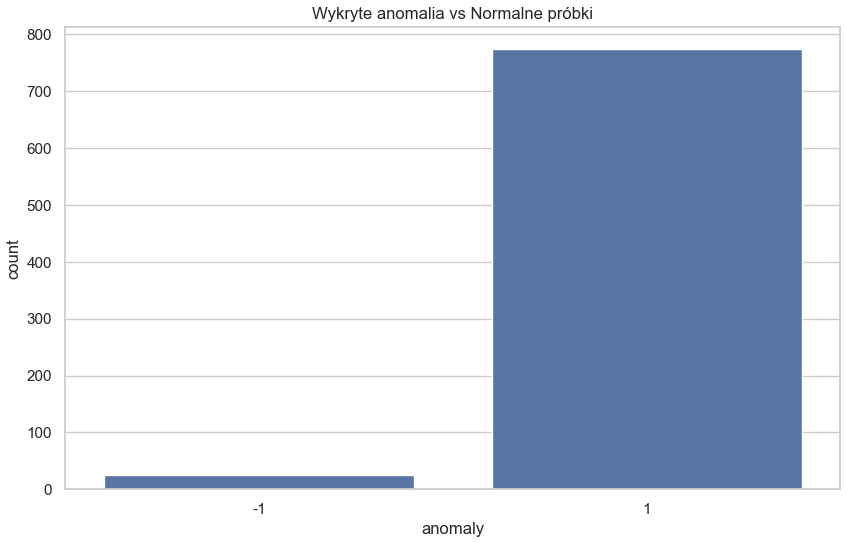
\includegraphics[scale=.50]{wykresy/wykres1.png}
	\caption{Wykryte anomalia vs Normalne próbki: -1: anomalia 1: normalny przypadek}
	\label{FIG:1}
\end{figure}

\begin{figure}[h]
	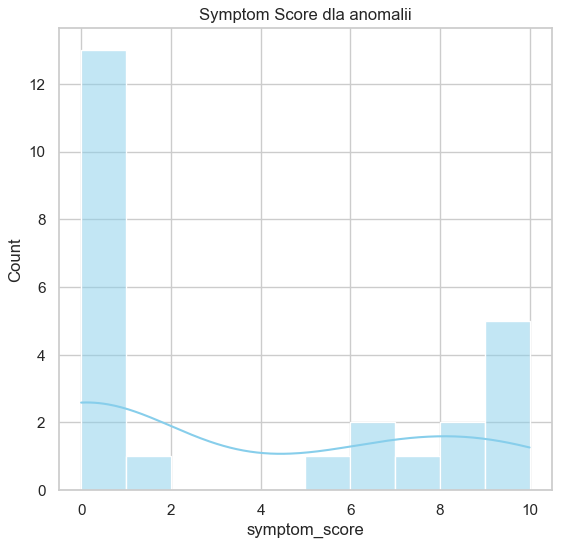
\includegraphics[scale=.70]{wykresy/wykres2.1.png}
	\caption{Rozkład ilości symptomów dla anomalii}
	\label{FIG:1}
\end{figure}
\newpage
.
\newpage
\begin{figure}[h]
	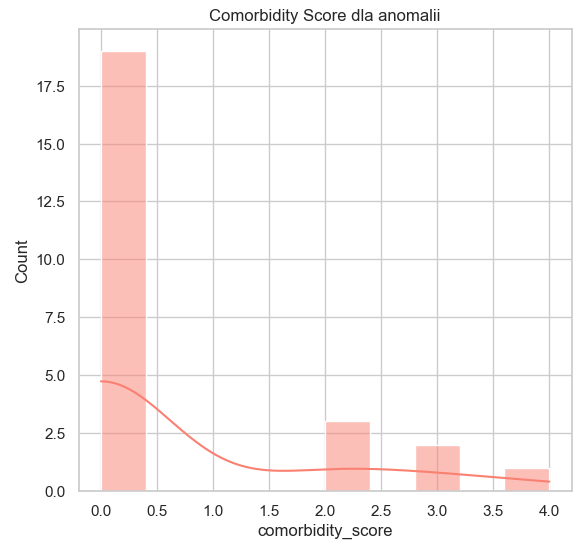
\includegraphics[scale=.60]{wykresy/wykres2.2.png}
	\caption{ Rozkład ilości chorób wspóistniejących dla anomalii}
	\label{FIG:1}
\end{figure}

\begin{figure}[h]
	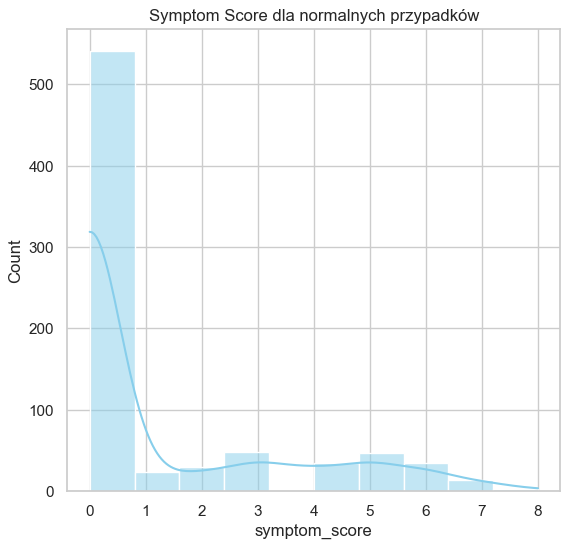
\includegraphics[scale=.60]{wykresy/wykres3.1.png}
	\caption{Rozkład ilości symptomów dla przypadków normalnych}
	\label{FIG:1}
\end{figure}
\newpage
.
\newpage
\begin{figure}[h]
	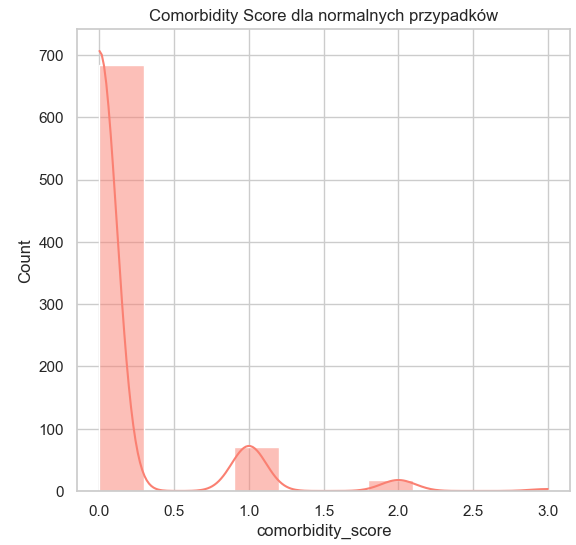
\includegraphics[scale=.53]{wykresy/wykres3.2.png}
	\caption{Rozkład ilości chorób wspóistniejących dla przypadków normalnych}
	\label{FIG:1}
\end{figure}

\begin{figure}[h]
	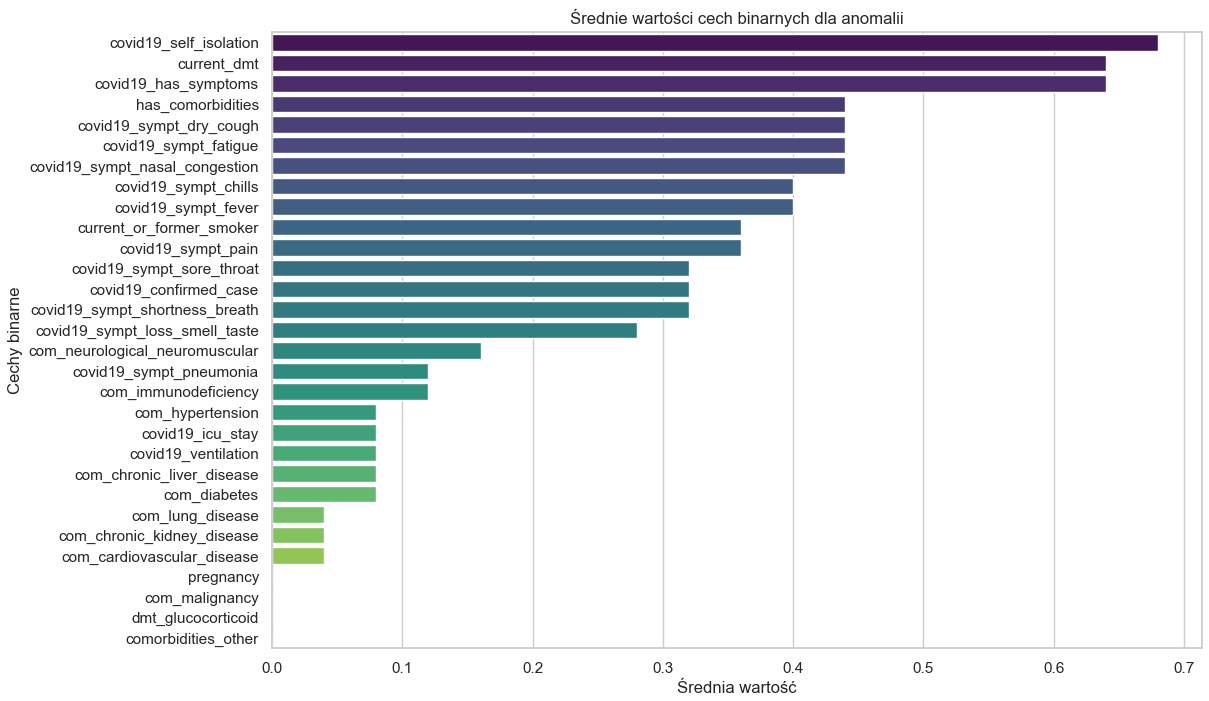
\includegraphics[scale=.53]{wykresy/wykres4.png}
	\caption{Średnie wartości charakterystycznych cech dla anomalii}
	\label{FIG:1}
\end{figure}
\newpage
.
\newpage
\begin{figure}[h]
	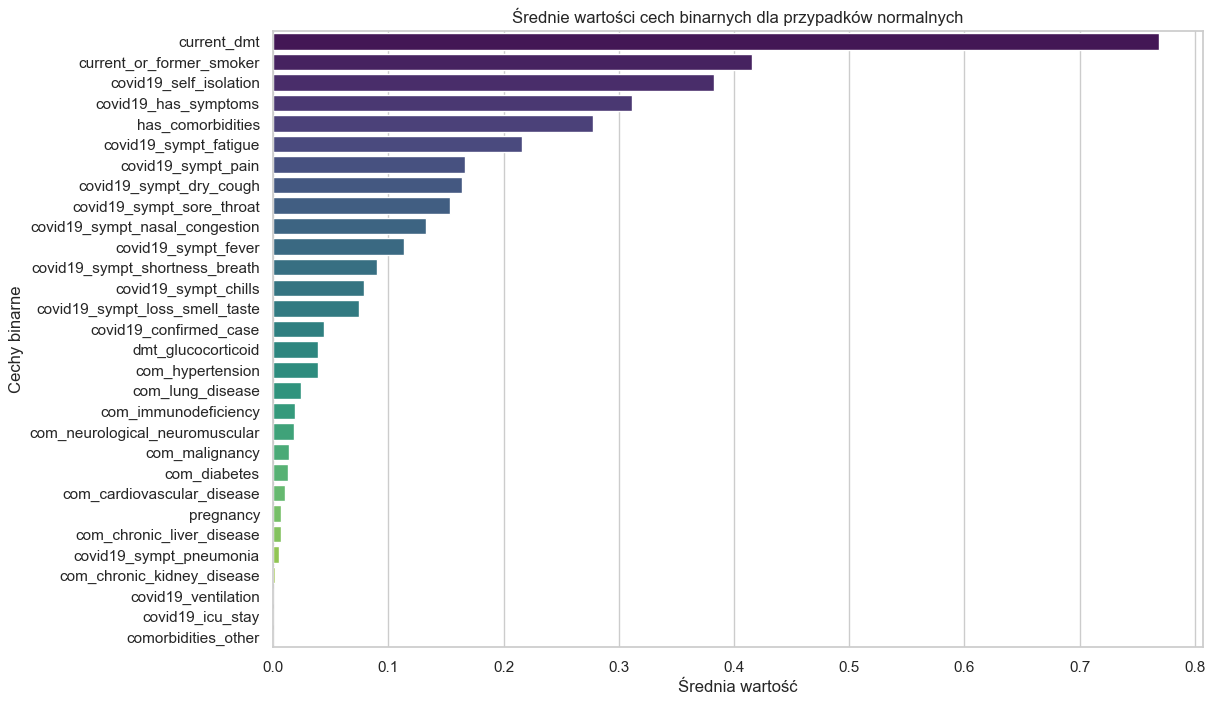
\includegraphics[scale=.53]{wykresy/wykres5.png}
	\caption{Średnie wartości charakterystycznych cech dla przypadków normalych}
	\label{FIG:1}
\end{figure}

\begin{figure}[h]
	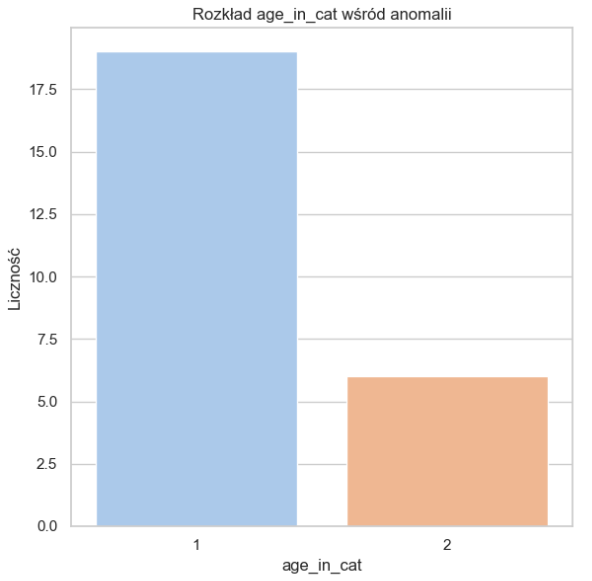
\includegraphics[scale=.46]{wykresy/wykres6.png}
	\caption{Rozkład wieku wśród anomalii: 0: jeśli zakres wieku mieści się w przedziale od 0 do <18. 
1: jeżeli przedział wiekowy mieści się w przedziale od 18 do <=50 lat.
2: jeżeli przedział wiekowy mieści się w przedziale od 51 do <=70 lat.
3: jeśli przedział wiekowy wynosi 71 lat lub więcej..}
	\label{FIG:1}
\end{figure}
\newpage
.
\newpage
\begin{figure}[h]
	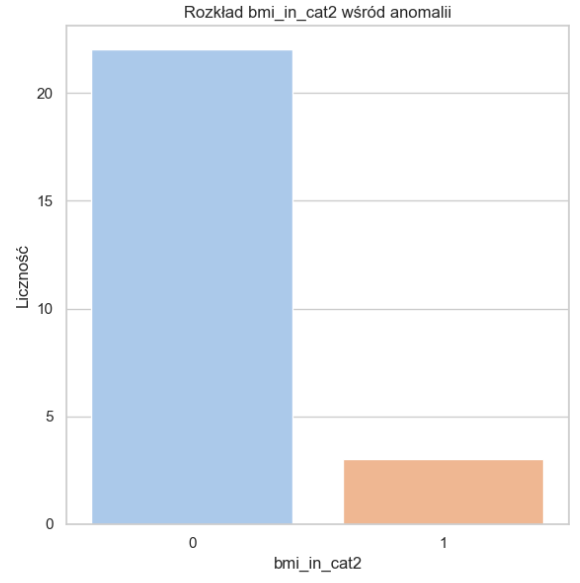
\includegraphics[scale=.57]{wykresy/wykres7.png}
	\caption{Rozkład bmi wśród anomalii: 0: not\_overweight: if BMI <= 30 kg/m2 
1: overweight: if BMI > 30 kg/m2.}
	\label{FIG:1}
\end{figure}

\begin{figure}[h]
	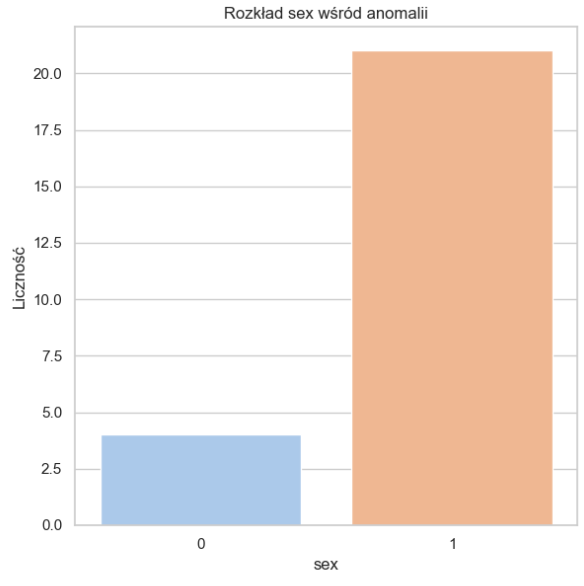
\includegraphics[scale=.57]{wykresy/wykres8.png}
	\caption{Rozkład płci wśród anomalii: 0: mężczyźni 1: kobiety}
	\label{FIG:1}
\end{figure}
\newpage
.
\newpage
\begin{figure}[h]
	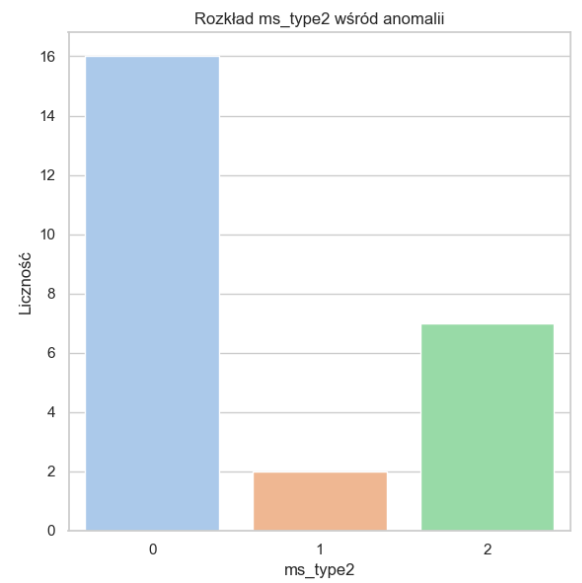
\includegraphics[scale=.80]{wykresy/wykres9.png}
	\caption{Rozkład typu stwardnienia rozsianego wśród anomalii:  0: relapsing\_remitting: jeśli typ stwardnienia rozsianego to stwardnienie rozsiane rzutowo-remisyjne (RRMS)
1: progresywny\_MS: jeśli typ stwardnienia rozsianego to wtórnie postępujące stwardnienie rozsiane (SPMS) lub pierwotnie postępujące stwardnienie rozsiane (PPMS)
2: inny: jeśli typ stwardnienia rozsianego to zespół izolowany klinicznie (CIS) lub pusty lub „niepewny”, w przypadku gdy pacjent lub lekarz nie był pewien.}
	\label{FIG:1}
\end{figure}
\newpage
.
\newpage
\begin{figure}[h]
	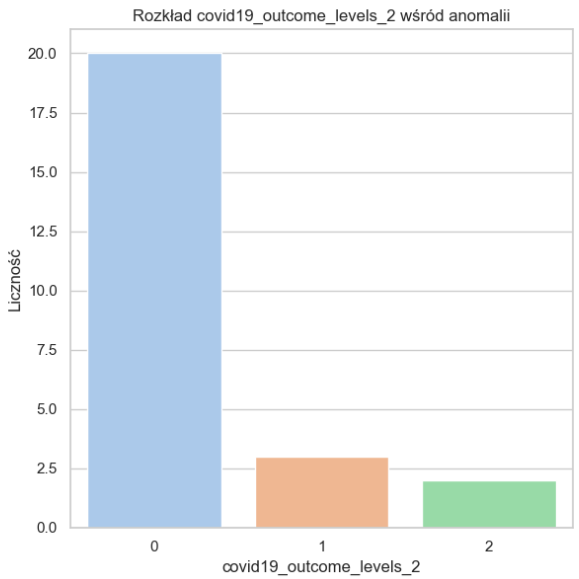
\includegraphics[scale=.80]{wykresy/wykres10.png}
	\caption{Rozkład hospitalizowanych przypadków: 0: Jeśli dana osoba ma Covid-19, ale nie była hospitalizowana.
1: Osoba ma Covid-19 i została hospitalizowana.
2: Osoba ma Covid-19, była hospitalizowana, przebywała na oddziale intensywnej terapii i/lub przebywała w ośrodku wentylacyjnym.
3: Osoba zmarła z powodu Covid-19 (nieobecna w tym zbiorze danych).}
	\label{FIG:1}
\end{figure}




\end{document}

